% Revisión interna; compilar con ./build_pdf.sh review y conservar .tex y PDF juntos.
\documentclass[11pt,letterpaper]{article}
\usepackage[utf8]{inputenc}
\usepackage[T1]{fontenc}
\usepackage{lmodern,microtype}
\usepackage[spanish,es-nodecimaldot,es-tabla]{babel}
\usepackage{amsmath,amssymb,array,booktabs,longtable,float,graphicx,caption}
\usepackage[hidelinks]{hyperref}
\usepackage[margin=1in]{geometry}
\graphicspath{{../../results/figures/}}
\setlength{\emergencystretch}{2em}
\let\originalunderscore\_
\renewcommand{\_}{\originalunderscore\allowbreak}
\title{Trabajo práctico 2: revisión del proyecto\\[0.5ex]\large Lógica, pasos, resultados y decisiones}
\author{Alejandro Quesada \and Jose Herrera \and Manfred Azofeifa}
\date{24 de octubre de 2026}
\begin{document}
\maketitle
\begin{abstract}
Revisión interna del detector de spam: recoge la implementación en un único
cuaderno, la auditoría del dataset, el modelo con sesgo y la evaluación de
regresión logística con y sin PCA. Los resultados anteriores de MiniLM con
384 características no describen el nuevo codificador MPNet con 768 ni el
protocolo de validación corregido. Se completaron 30 corridas por cada una
de las cuatro variantes de regresión con MPNet. El punto 2 está completo:
el detector de histogramas usa 2 componentes, elegidas en validación interna
porque con 384 el spam resulta más verosímil que el ham. En 30 corridas
obtiene F1 0.7043, frente a 0.9641 de la regresión sin PCA. Este documento se mantiene junto con
\texttt{TODO.md}, \texttt{AGENTS.md} y su PDF compilado.
\end{abstract}
\tableofcontents
\newpage

\section{Alcance y organización}
El enunciado pide detectar spam de SMSSpamCollection (UCI) mediante regresión
logística propia, detección de anomalías por histogramas y modelos grandes de
lenguaje. La entrega indicada en el enunciado es el 20 de octubre de 2026.

Desde el 24 de octubre se concentra toda la implementación en
\texttt{notebooks/tp2\_detector\_spam.ipynb}: utilidades, funciones de los tres
puntos, experimentos y análisis. Se retira la regla de un archivo por punto y
el paquete \texttt{src/tp2/}. Se conserva la organización por apartados dentro
del cuaderno, sin copias de las funciones en archivos Python.

\begin{center}
\begin{tabular}{p{0.38\linewidth}p{0.55\linewidth}}
\toprule
\textbf{Ubicación} & \textbf{Responsabilidad}\\
\midrule
Cuaderno principal & Definiciones, configuración, ejecución y análisis en
celdas diferenciadas.\\
\texttt{tests/} & Pruebas externas que ejecutan las definiciones del cuaderno.\\
\texttt{docs/report/sections/} & Informe LaTeX, organizado por punto.\\
\texttt{results/} & Figuras y tablas producidas por el cuaderno.\\
\texttt{data/raw/} & Dataset original versionado, sin modificaciones.\\
\texttt{data/processed/} & Cachés regenerables, excluidas de Git.\\
\bottomrule
\end{tabular}
\end{center}

Las celdas reutilizables comienzan por \texttt{\# Definiciones:}.
\texttt{tests/notebook\_loader.py} las ejecuta en orden en un espacio de
nombres común, sin ejecutar descargas, configuración de exportación ni
experimentos. Así las pruebas comprueban la implementación que se entrega.
Las dependencias opcionales se importan dentro de las funciones que las usan.

Se mantienen los contratos: características \texttt{float32} de forma
$(n,D)$; etiquetas y predicciones \texttt{int64} de forma $(n,)$; ham $=0$,
spam $=1$ y spam como clase positiva del F1. Las funciones reciben datos y
parámetros explícitamente y llevan documentación Doxygen en español.

\section{Auditoría del dataset y sus dimensiones}
El archivo local \texttt{data/raw/SMSSpamCollection} coincide byte por byte
con el del ZIP oficial de UCI. Su SHA256 es
\texttt{7d039a24a6083ed9ef0f806ebad56bbb9\allowbreak 76e3aeb8de05669173bfdc4996c239d}.
Tiene 5574 filas: 4827 ham y 747 spam. Cada fila contiene etiqueta y texto;
no contiene 768 columnas de características. No hay mensajes vacíos ni errores
de UTF-8. Hay 5171 textos únicos y 403 repeticiones adicionales, sin etiquetas
contradictorias para un mismo texto.

\paragraph{De dónde sale $D$.} El codificador anterior,
\texttt{sentence-transformers/all-MiniLM-L6-v2}, produce 384 características.
El equipo confirmó cambiar a
\texttt{sentence-transformers/all-mpnet-base-v2}, que produce 768. Las fichas
oficiales describen ambas dimensiones:
\href{https://huggingface.co/sentence-transformers/all-MiniLM-L6-v2}{MiniLM}
y \href{https://huggingface.co/sentence-transformers/all-mpnet-base-v2}{MPNet}.
La dimensión depende del codificador; cambiarla exige recalcular
características, calibración, métricas, tablas y figuras.

\paragraph{Limitación de duplicados.} Se conserva el archivo original y el
protocolo estratificado por filas. Por ello un texto idéntico puede aparecer
en entrenamiento y prueba, lo que limita la interpretación como generalización
a mensajes nuevos. Una evaluación agrupada por texto sería otro protocolo y
requiere acordarla con el equipo; no se deduplicó silenciosamente.

\section{Puntos 1.1 y 1.2: modelo básico con sesgo}
El enunciado pide regresión logística. La confirmación del equipo mantiene
una parte lineal básica con sesgo y una sigmoide:
\[
 z=Xw+b,\qquad p(y=1\mid x)=\sigma(z).
\]
\texttt{forward} calcula probabilidades; el sesgo es un escalar entrenable.
La sigmoide se evalúa con $e^{-|z|}$ para evitar desbordamientos con logits
extremos. El entrenamiento propio minimiza la entropía cruzada binaria media
con descenso del gradiente por lotes completos:
\[
 \nabla_w L=X^\top(p-y)/n,\qquad \partial L/\partial b=\overline{p-y}.
\]
Se actualizan tanto $w$ como $b$. No se utilizan \texttt{torch.nn},
optimizadores de \texttt{torch.optim} ni clasificadores ya implementados.
La pérdida se calcula a partir de logits de forma estable. El historial
conserva la pérdida inicial y una por época.

Las cuatro pruebas obligatorias verifican probabilidades con pesos nulos,
sigmoide y estabilidad extrema, primer paso de gradiente (incluido el sesgo)
y clasificación reproducible de datos separables. En pruebas se permite
Autograd como referencia independiente.

\section{Punto 1.3: demostración aislada}
El conjunto sintético bidimensional verifica el entrenamiento y la evolución
de su frontera frente a una recta conocida con sesgo. Se conservan sus propias
semillas, tasa y épocas. Sus datos, modelo e hiperparámetros no se usan en
1.4, 1.5 ni 2: esos apartados trabajan exclusivamente con los mensajes UCI y
sus características. Las funciones genéricas \texttt{forward} y de
entrenamiento son compartidas; los resultados experimentales no lo son.

\section{Punto 1.4: extracción y evaluación corregidas}
Se codifica cada mensaje original con MPNet y se verifica forma $(5574,768)$,
tipo \texttt{float32}, orden de las filas y valores finitos. La caché identifica
el dataset y el codificador para impedir reutilizar características de otro
modelo o archivo. El codificador preentrenado no se ajusta sobre UCI, así que
la extracción puede realizarse una vez antes de las particiones.

\subsection{Validación dentro de cada corrida}
Se mantienen 30 particiones estratificadas 70\,\%/30\,\%, con semillas
$2026,\ldots,2055$. En cada una:
\begin{enumerate}
\item Se reserva el 30\,\% para prueba y no se usa al seleccionar parámetros.
\item Se divide el entrenamiento en 80\,\% de ajuste y 20\,\% de validación.
\item Se prueban tasas $\{0.1,0.5,1,2,5,10,20,50\}$ y épocas
$\{250,500,1000,2000,4000\}$. Se elige mayor F1 de validación y, en caso de
empate, menor pérdida de validación.
\item Se aplica automáticamente la combinación ganadora al entrenar un modelo
nuevo sobre todo el 70\,\% de entrenamiento; se evalúa una vez en su prueba.
\end{enumerate}

Antes se calibraba una sola vez con la primera partición y se reutilizaba
la elección en las otras 29. Esa validación incluía 244 mensajes que luego
estaban en la prueba de la semilla 2027 y 226 de la semilla 2028. Por tanto
esas pruebas no estaban aisladas de la selección global. No se puede afirmar
que el sesgo fuera pequeño sin medirlo. Además, la calibración solo imprimía
una advertencia si su ganador no coincidía con las constantes manuales; ahora
se consume el ganador directamente.

% RESULTADOS_14
\subsection{Resultados de la nueva ejecución}
Se ejecutaron las 30 corridas completas con MPNet/768, antes de ejecutar la
demostración 1.3: la evaluación no necesita sus datos ni su entrenamiento.
Las cifras son medias y desviaciones muestrales entre corridas.
\begin{center}
\begin{tabular}{lrrrr}
\toprule
Métrica & Media & Desviación & Mínimo & Máximo\\
\midrule
Tasa de aciertos & 0.9906 & 0.0016 & 0.9874 & 0.9940\\
F1 & 0.9641 & 0.0063 & 0.9519 & 0.9776\\
\bottomrule
\end{tabular}
\end{center}
En la primera corrida la validación eligió tasa 20 y 4000 épocas, con F1
0.9714. Es un ejemplo de selección interna, no una constante para las demás
corridas: sus elecciones se registran en la tabla exportada de hiperparámetros.
La mejora frente a cifras históricas no permite atribuir el cambio solo al
codificador, porque también se corrigió el protocolo de selección.
\begin{figure}[H]
\centering
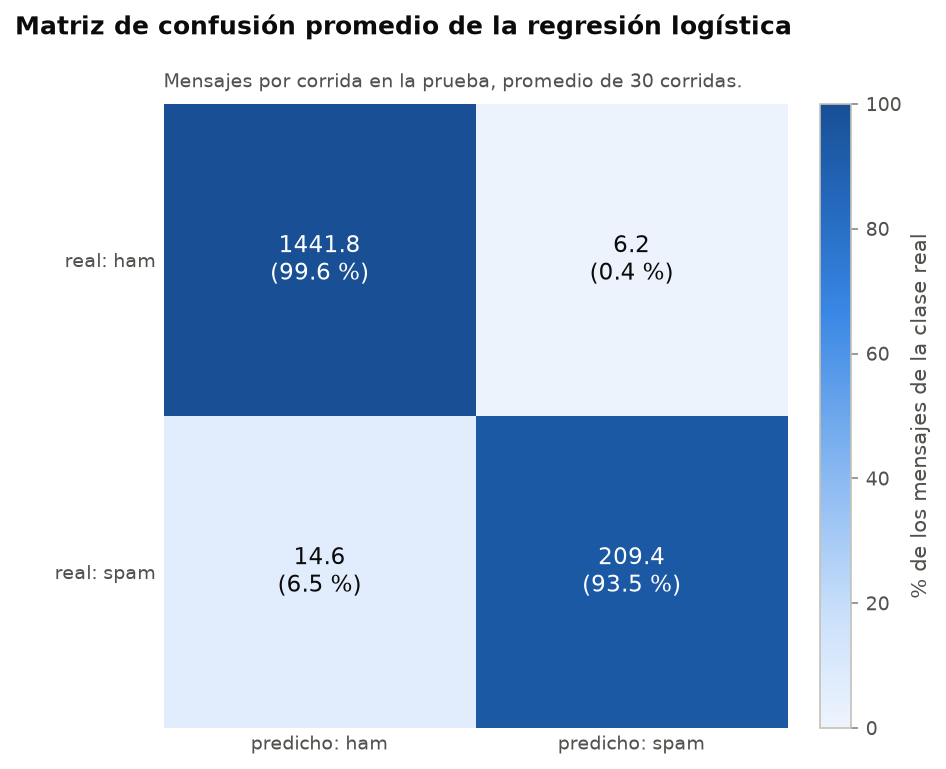
\includegraphics[width=0.86\linewidth]{matriz-de-confusion-promedio-de-la-regresion-logistica.png}
\caption{Errores medios de las 30 pruebas con MPNet/768, después de la
calibración interna de cada corrida.}
\end{figure}
% FIN_RESULTADOS_14

\section{Punto 1.5: reducción y comparación con PCA}
Con $D=768$ se comparan $k=384$ (50\,\%), $k=192$ (25\,\%) y $k=2$ con el
caso sin PCA. Se conserva PCA propio por SVD de datos centrados, cálculo en
doble precisión y signo fijo de cada componente. La proyección recibe la
media y componentes obtenidas del conjunto de ajuste correspondiente.

La calibración se repite para cada corrida y cada $k$. Durante la selección,
el PCA se ajusta solo con el ajuste interno y transforma la validación.
Tras elegir tasa y épocas se reajusta PCA sobre todo el entrenamiento
externo; se entrena allí y se transforma la prueba sin reajustarlo.
Comparar las mismas semillas permite calcular diferencias pareadas de F1.
Las proyecciones y la varianza de todo el dataset son diagnósticos descriptivos,
no criterios para consultar la prueba al elegir hiperparámetros.

% RESULTADOS_15
\subsection{Resultados y dimensión óptima}
Se completaron las 90 corridas con PCA y las 30 sin PCA, con las mismas
semillas. La varianza corresponde al PCA descriptivo sobre todo el dataset;
las métricas usan únicamente PCA ajustados con el entrenamiento correspondiente.
\begin{center}
\begin{tabular}{rrrrr}
\toprule
$k$ & Varianza & Tasa de aciertos & F1 & $\Delta$ F1 pareado\\
\midrule
768 & 100\,\% & $0.9906\pm0.0016$ & $0.9641\pm0.0063$ & ---\\
384 & 96.16\,\% & $0.9905\pm0.0019$ & $0.9637\pm0.0075$ & $-0.0004$\\
192 & 84.13\,\% & $0.9894\pm0.0021$ & $0.9596\pm0.0082$ & $-0.0045$\\
2 & 8.08\,\% & $0.9466\pm0.0054$ & $0.7845\pm0.0189$ & $-0.1796$\\
\bottomrule
\end{tabular}
\end{center}
Con 384 componentes el F1 es menor que sin PCA en 14 de las 30 particiones;
la diferencia pareada es $-0.0004\pm0.0030$. Con 192, baja en 24 de las 30,
con diferencia $-0.0045\pm0.0054$. Con 2 baja en todas, con diferencia
$-0.1796\pm0.0198$: se escapan 61.4 spam por prueba frente a 11.8 sin PCA,
y los ham marcados como spam suben de 4.0 a 27.9.

Las 384 componentes conservan casi toda la varianza y un F1 medio próximo
al del caso completo. Las 192 vuelven a reducir a la mitad el número de
características con mayor pérdida media. Dos dimensiones sirven para
visualizar, pero pierden información relevante para clasificar. La desviación
entre particiones solapadas no es un intervalo de confianza de muestras
independientes. No se atribuye significación estadística a la diferencia pequeña
con 384 componentes.

\begin{figure}[H]
\centering
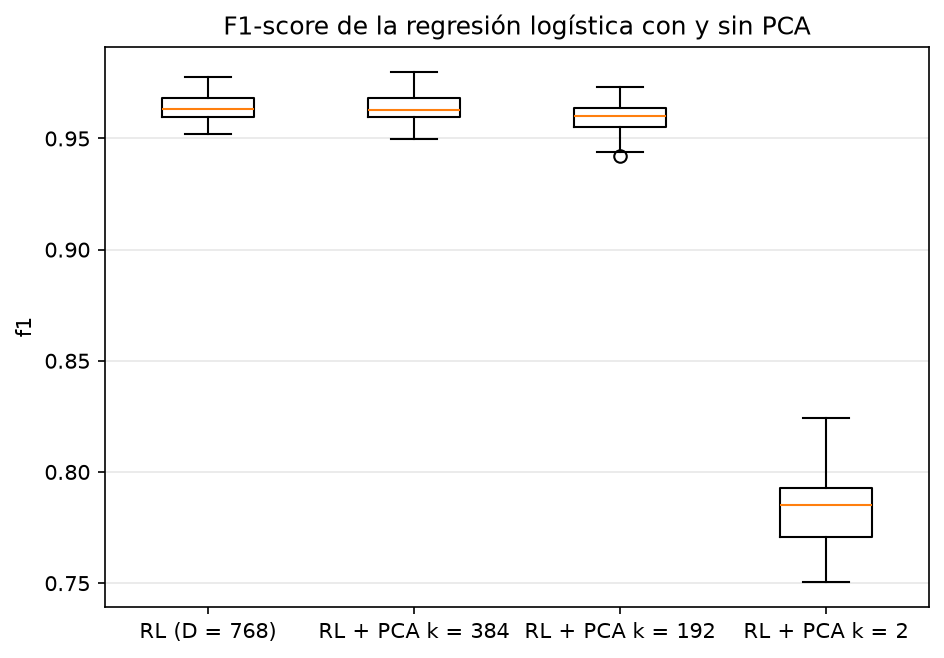
\includegraphics[width=0.96\linewidth]{f1-score-de-la-regresion-logistica-con-y-sin-pca.png}
\caption{F1 en las mismas 30 particiones, con validación interna por método y corrida.}
\end{figure}

El equipo confirmó \texttt{OPTIMAL\_PCA\_DIMENSIONS = 384} el 24 de octubre
de 2026. Se reduce a la mitad la dimensión inicial de MPNet y se conserva
el 96.16\,\% de la varianza descriptiva. El F1 medio es 0.9637 frente a
0.9641 sin PCA, con diferencia media pareada de $-0.0004$. Esta cercanía
no demuestra equivalencia estadística; se adopta como compromiso entre
reducción y clasificación observada para la regresión logística. La decisión
se basa en MPNet/768 y no en las recomendaciones anteriores de MiniLM/384.
El detector del punto 2 compara estos mismos casos con su propia validación
(Sección~\ref{sec:review-punto21}).
% FIN_RESULTADOS_15

\section{Punto 2.1: densidades por histograma y umbral}
\label{sec:review-punto21}
\paragraph{Lógica.} En cada partición se ajusta un PCA solo con el
entrenamiento. Por componente se estima un histograma de 30 intervalos de
igual ancho entre el mínimo y el máximo de los datos, normalizado para que
integre 1. El puntaje es $\sum_d\log p_d(x_d)$; un valor en un intervalo vacío
o fuera del soporte recibe $\varepsilon=10^{-12}$ ($\log\varepsilon\approx-27.6$)
sin recortar el dato. Un puntaje menor que el umbral marca spam.

\paragraph{Pasos.}
\begin{enumerate}
\item Se implementaron \texttt{fit\_histogram\_densities},
\texttt{per\_dimension\_log\_likelihood}, \texttt{log\_likelihood},
\texttt{select\_threshold} (cuantil con interpolación lineal) y las gráficas,
hasta superar las nueve pruebas ya escritas para el 2.1.
\item \texttt{fit\_anomaly\_detector} reparte los ham del entrenamiento: el
80\,\% construye los histogramas y el 20\,\% reservado da los puntajes del
cuantil 5\,\%. Si el umbral sale de los mismos ham de los histogramas, ninguno
cae fuera del soporte y el umbral queda sesgado. En la primera partición, con
384 componentes, quedaba marcado el 17.3\,\% de los ham de prueba en lugar del
5\,\% (7.9\,\% con ham reservado); con 2 componentes el efecto es menor: 5.9\,\%
frente a 4.4\,\%.
\item Con 384 componentes el detector casi no encuentra spam. Se diagnosticó
con la brecha por componente (media de $\log p_d$ de ham menos la de spam) y
se compararon los casos de 1.5 en la validación interna de los 30
entrenamientos, sin usar la prueba.
\item Se agregaron cinco pruebas: suma por dimensión, umbral con filas
reservadas, candidatos con columnas iniciales y solo ham, signo de la brecha
y títulos de las figuras nuevas.
\end{enumerate}

\paragraph{Resultados de la selección.} Validación interna (20\,\% estratificado
del entrenamiento, como en 1.4) de las 30 particiones; media $\pm$ desviación:
\begin{center}
\begin{tabular}{rrrrrr}
\toprule
$D$ & Tasa de aciertos & F1 & Spam detectado & Ham marcado & Gana\\
\midrule
384 & $0.7810\pm0.0140$ & $0.0401\pm0.0193$ & 3.4\,\% & 10.3\,\% & 0\\
192 & $0.8425\pm0.0072$ & $0.0237\pm0.0191$ & 1.4\,\% & 2.9\,\% & 0\\
2 & $0.9201\pm0.0106$ & $0.7085\pm0.0318$ & 72.1\,\% & 4.9\,\% & 30\\
\bottomrule
\end{tabular}
\end{center}
En la primera partición, la brecha de la componente~1 es 12.8 y es negativa
en 330 de las 384 componentes: el spam está más concentrado que el ham y
recibe más densidad. La brecha acumulada vale $+12.6$ con 2 componentes,
cruza cero en 169, vale $-2.8$ con 192 y $-41.1$ con 384. Su máximo (14.2,
con 11) no se evaluó porque el enunciado limita la elección a las dimensiones
de 1.5.

\begin{figure}[H]
\centering
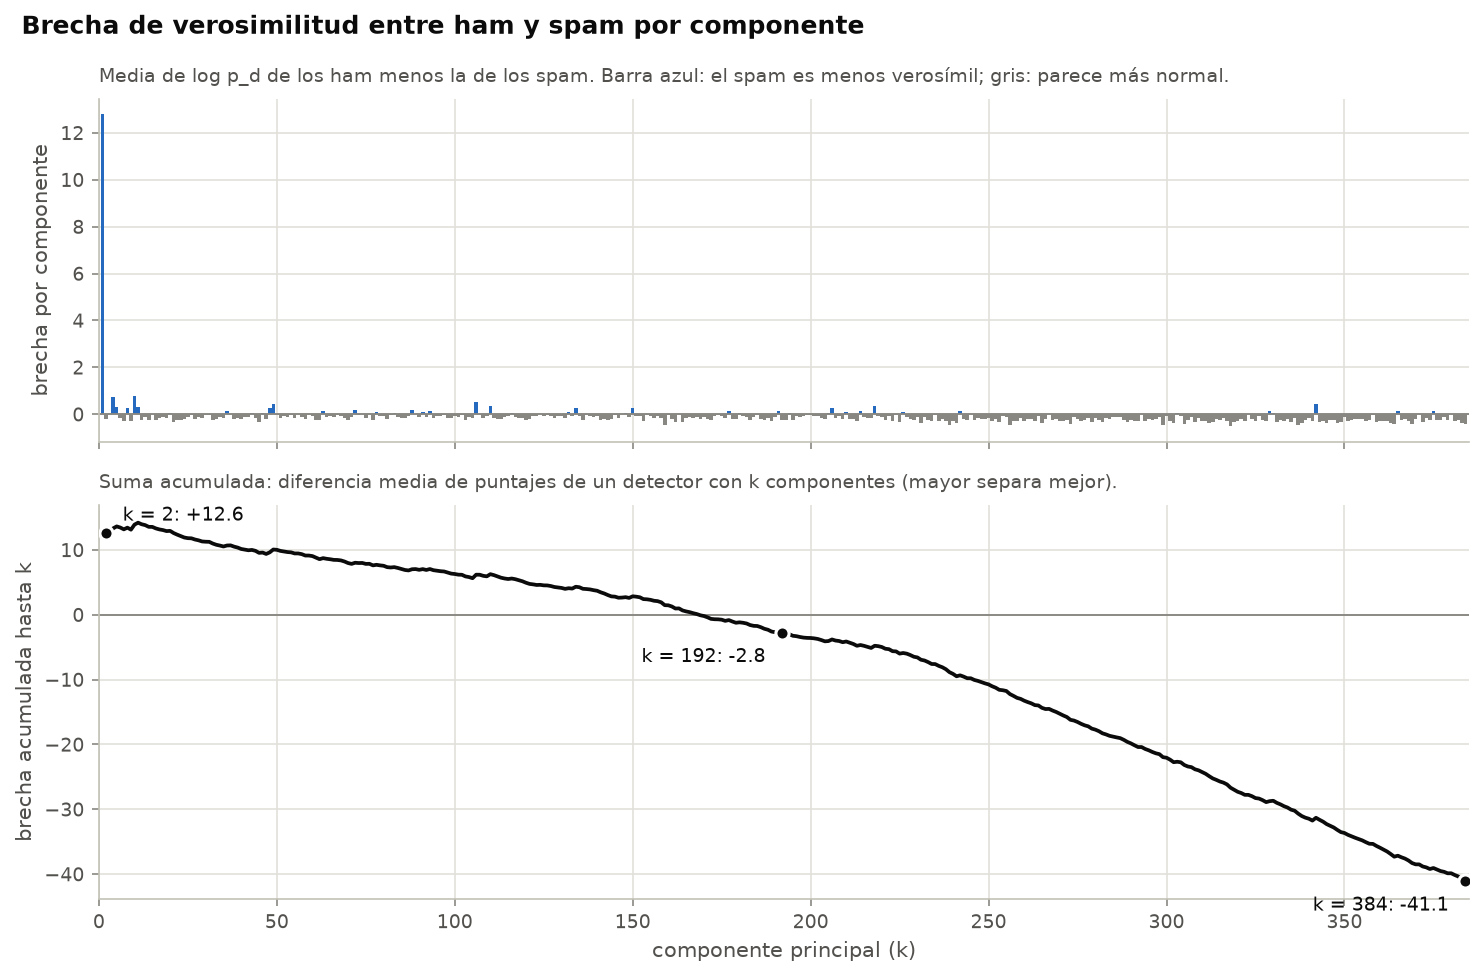
\includegraphics[width=0.86\linewidth]{brecha-de-verosimilitud-entre-ham-y-spam-por-componente.png}
\caption{Brecha de verosimilitud por componente y acumulada (primera partición, validación).}
\end{figure}

\paragraph{Demostración con $D=2$.} Semilla 2026: 2703 ham construyen los
histogramas, 676 fijan el umbral $\tau=-0.8334$. En su prueba queda bajo el
umbral el 4.4\,\% de los ham y el 75.9\,\% del spam (tasa de aciertos 0.9294,
F1 0.7424). El 50\,\% del spam queda fuera del soporte de la componente~1 y
el 25.9\,\% cae en zonas de baja densidad; el resto se mezcla con el ham.

\begin{figure}[H]
\centering
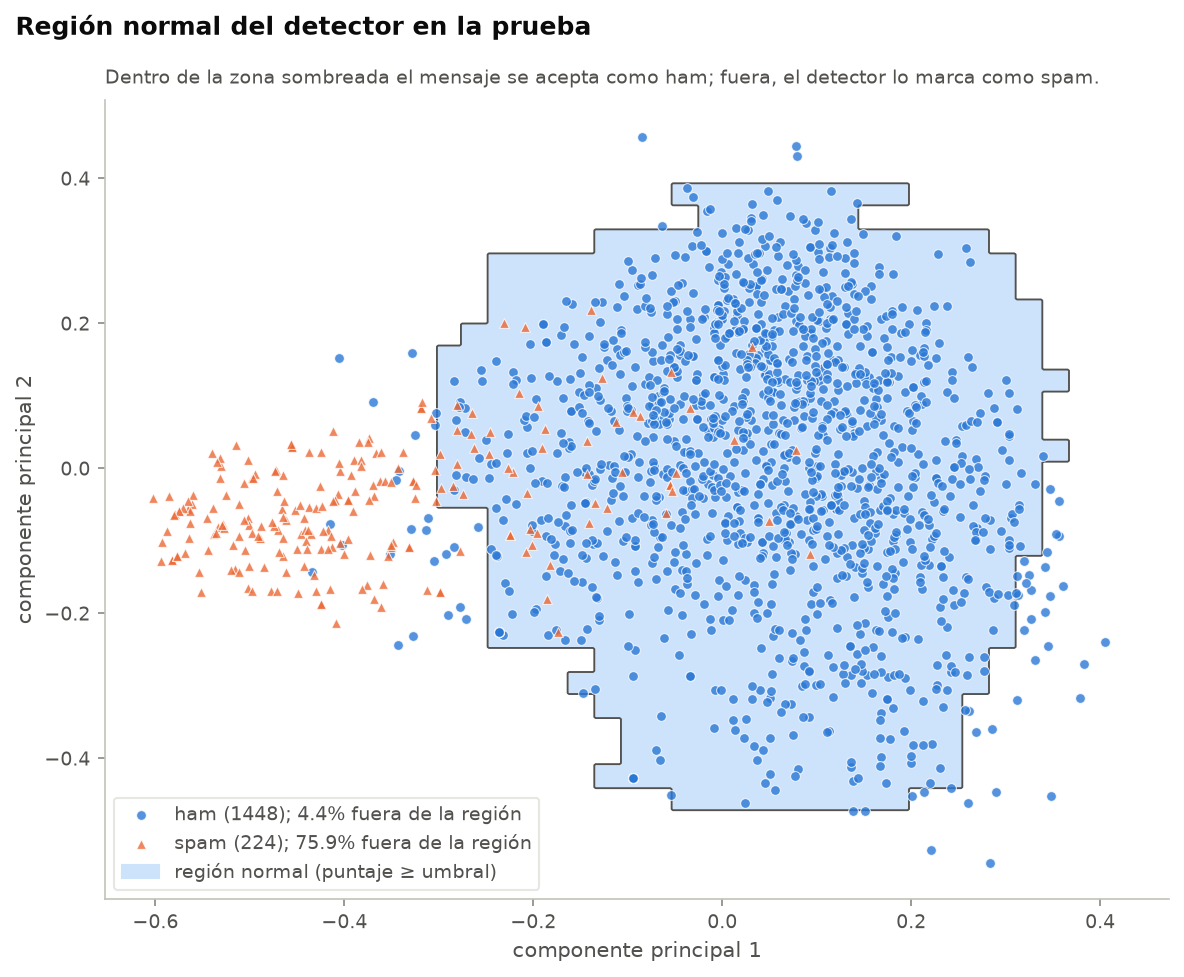
\includegraphics[width=0.62\linewidth]{region-normal-del-detector-en-la-prueba.png}
\caption{Región normal del detector con $D=2$ y mensajes de prueba (semilla 2026).}
\end{figure}

\section{Punto 2.2: evaluación en 30 corridas}
\paragraph{Pasos.} La celda del 2.2 repite el detector del 2.1 en las 30
particiones de la regresión (semillas 2026--2055), con PCA, histogramas y
umbral ajustados solo con cada entrenamiento. Además de la tabla de medias,
compara corrida a corrida con la regresión sin PCA y con la regresión de
$k=2$, y reporta los errores por clase. Para tener los resultados por
partición del punto~1 se volvieron a ejecutar sus 120 corridas en esta
máquina: las tablas de métricas coinciden exactamente con las versionadas.

\paragraph{Resultados.} Media $\pm$ desviación; errores promedio por prueba
(1448 ham y 224 spam):
\begin{center}
\begin{tabular}{lrrrr}
\toprule
Método & Tasa de aciertos & F1 & Ham marcado & Spam detectado\\
\midrule
Regresión, 768 & $0.9906\pm0.0016$ & $0.9641\pm0.0063$ & 4.0 & 94.7\,\%\\
Regresión, $k=2$ & $0.9466\pm0.0054$ & $0.7845\pm0.0189$ & 27.9 & 72.6\,\%\\
Histogramas, $D=2$ & $0.9195\pm0.0084$ & $0.7043\pm0.0247$ & 70.5 & 71.4\,\%\\
\bottomrule
\end{tabular}
\end{center}
Diferencia pareada de F1 del detector: $-0.2597\pm0.0253$ frente a la
regresión sin PCA y $-0.0802\pm0.0212$ frente a $k=2$; menor en las 30
corridas en ambos casos. El F1 de validación del 2.1 (0.7085) anticipó el de
prueba (0.7043). Con 2 componentes, ambos métodos detectan casi el mismo
spam; el detector marca más ham (4.9\,\% contra 1.9\,\%) porque su umbral
acepta el 5\,\% de los ham y no sabe hacia dónde está el spam.

\begin{figure}[H]
\centering
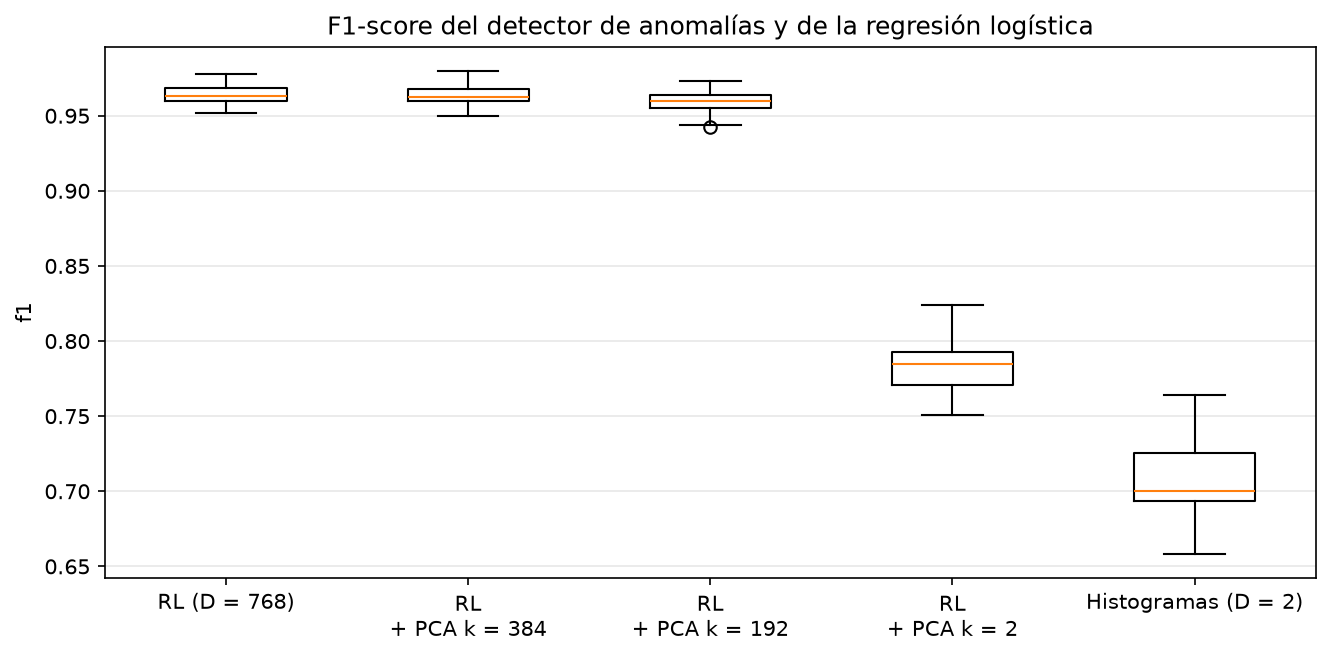
\includegraphics[width=0.8\linewidth]{f1-score-del-detector-de-anomalias-y-de-la-regresion-logistica.png}
\caption{F1 del detector y de la regresión en las mismas 30 particiones.}
\end{figure}

\section{Puntos pendientes}
El punto 2 está completo. Lo que falta, en orden (detalle en \texttt{TODO.md}):
\begin{enumerate}
\item Ejecutar el cuaderno completo desde un kernel limpio: las celdas del
punto 2 se ejecutaron en un entorno aparte y no tienen salidas; la tabla
exportada de pruebas sigue en 30/2/0 (\texttt{pytest} da 44/1/0) y la figura
de F1 del 1.5 debe regenerarse con las etiquetas nuevas. La configuración
borra las exportaciones; sin caché, la extracción de MPNet en CPU con un hilo
tarda más de 10 minutos.
\item Avisar al equipo que el detector usa 2 componentes y la regresión 384.
\item Punto 3: elegir modelos, prompt y tratamiento de respuestas ambiguas;
LoRA o DoRA como extra. Sus tareas y pruebas no se eliminan.
\item Completar la comparación de métodos y las conclusiones del informe.
\item Confirmar integrantes y fecha de entrega (el enunciado indica el 20
de octubre); luego Doxygen, PDF final y \texttt{.zip}.
\item Menor: llevar los diagramas de caja al estilo común de las gráficas.
\end{enumerate}

\newpage
\section{Registro de decisiones}
\small
\begin{longtable}{p{0.14\linewidth}p{0.38\linewidth}p{0.39\linewidth}}
\toprule
\textbf{Fecha} & \textbf{Decisión} & \textbf{Motivo}\\
\midrule\endhead
17/10/2026 & Sigmoide estable y gradiente exacto propio. & Implementación
transparente sin desbordamientos ni optimizadores externos.\\
19/10/2026 & Frontera verdadera fija en 1.3. & Comparar la recta aprendida
con una referencia con sesgo.\\
23/10/2026 & 1.3 independiente de UCI; dataset original versionado. & Evitar
mezclar demostración sintética y evaluación real; compartir los mismos datos.\\
23/10/2026 & PCA por SVD centrada y comparación pareada. & Ajuste propio y
comparación sobre las mismas particiones.\\
24/10/2026 & Único notebook con toda la implementación. & Sustituye archivos
por punto y utilidades separadas; pruebas consumen las mismas definiciones.\\
24/10/2026 & Mantener logística $Xw+b$ seguida de sigmoide. & Confirmación del
equipo; coincide con 1.1 y 1.2 del enunciado.\\
24/10/2026 & MPNet con 768 características; descargar y ejecutar 1.4--1.5. &
Confirmación del equipo; reemplaza MiniLM/384 y sus resultados.\\
24/10/2026 & Calibración interna por corrida y cantidad de componentes. &
Aislar cada prueba y usar el ganador automáticamente.\\
24/10/2026 & Conservar duplicados y documentar su limitación. & Mantener el
dataset original y el protocolo por filas sin introducir otra evaluación.\\
24/10/2026 & Fijar $D=384$ para el punto 2. & Decisión del equipo: mitad de
las características, 96.16\,\% de varianza descriptiva y F1 medio 0.9637
frente a 0.9641 sin PCA; no implica equivalencia estadística.\\
24/10/2026 & Densidades del punto 2 solo con ham del entrenamiento. &
Describir la distribución normal; el spam queda como lo atípico.\\
24/10/2026 & Umbral: cuantil 5\,\% de un 20\,\% de ham reservado; 30
intervalos. & Con los ham de los histogramas el umbral queda sesgado hacia
arriba (con 384 componentes marcaba 17.3\,\% de ham en vez de 5\,\%).\\
24/10/2026 & Detector con $D=2$; la regresión conserva 384. & Mayor F1 de
validación interna en las 30 particiones entre los casos de 1.5; con 384 el
spam resulta más verosímil que el ham (F1 0.04).\\
24/10/2026 & 2.2: comparar el detector por partición con la regresión sin PCA
y con $k=2$. & Separar el efecto de la dimensión del efecto del método, con
las mismas semillas.\\
\bottomrule
\end{longtable}
\normalsize

\section{Verificación y reproducción}
% VERIFICACION_ACTUAL
\begin{itemize}
\item \texttt{pytest}: 44 pruebas superadas, 1 pendiente (3.1), 0
fallidas, en terminal.  La celda de pruebas del cuaderno no se volvió a
ejecutar en esta revisión. Incluye búsqueda vectorizada equivalente
al entrenamiento individual, aislamiento de prueba, PCA interno y rechazo
de cachés incompatibles.
\item Cuaderno guardado validado con \texttt{nbformat}, IDs únicos y análisis
sintáctico. Se conservan documentación Doxygen, sesgo y gradiente.
\item Dataset contrastado con el original UCI. Características MPNet
$(5574,768)$, finitas, \texttt{float32} y de norma 1. Las cuatro variantes
completaron 30 corridas con semillas 2026--2055. Toda la evaluación UCI se
completó antes de crear los datos sintéticos de 1.3.
\item La inspección estática del IDE no resuelve algunos imports de pruebas
y atributos del módulo cargado dinámicamente; su ejecución real y las pruebas
los verifican. El informe preliminar también compila (21 páginas), con el
punto 3 todavía pendiente.
\item Punto 2.1 ejecutado con las características MPNet en caché (forma
$(5574,768)$, misma revisión del codificador). Sus figuras y la tabla de
selección se exportaron sin reejecutar el punto 1, cuyos resultados no
cambiaron.
\item Punto 2.2: 30 corridas del detector. Para compararlas por partición se
volvieron a ejecutar las 120 corridas del punto~1 en Linux: sus tablas de
métricas coinciden exactamente con las versionadas. Solo difieren en el
séptimo decimal las pérdidas de calibración y, en la corrida 23 con $k=2$, un
empate resuelto con 1000 épocas en vez de 2000, sin cambio en sus métricas.
No se sobrescribieron los archivos del punto~1.
\item La función compartida de diagramas de caja parte en dos líneas los
nombres largos; la figura versionada del 1.5 conserva el formato anterior
hasta la próxima ejecución completa.
\item Figuras inspeccionadas visualmente y PDF compilado con
\texttt{./build\_pdf.sh review}. La ejecución final y Doxygen siguen pendientes,
al igual que el punto 3.
\end{itemize}
% FIN_VERIFICACION_ACTUAL

Para reproducir, instalar \texttt{requirements.txt} y ejecutar las definiciones,
configuración, datos y punto 1 completos del cuaderno. La configuración limpia
las exportaciones: regenerar las figuras antes de compilar documentos que las usen.

\end{document}
